I dispositivi di networking sono la base della costruzione di una rete di telecomunicazioni moderna.
Si dividono in diverse categorie:
\begin{itemize}
	\item Dispositivi per forwarding e routing (switch, router)
	\item Dispositivi per garantiscono altri tipi di funzionalità (middlebox) come firewall, proxy, load balancer, ecc.
\end{itemize}
In generale questi tipi di dispositivi condividono alcuni aspetti, ad esempio includono:
\begin{itemize}
	\item \textbf{Data plane}: gestisce i pacchetti in modo locale, in generale si occupa di operazioni facili che devono essere eseguite ad alta velocità.
	\item \textbf{Control plane}: gestisce le operazioni di controllo e operazioni che permettono il corretto funzionamento della rete nel suo complesso.
	In generale queste operazioni sono più complesse e non devono essere eseguite ad alta velocità.
\end{itemize}


\section{Dispositivi per il forwarding e routing}
\subsection{Router}
\begin{itemize}
	\item \textbf{Data plane}:
	\begin{itemize}
		\item Quando un pacchetto arriva viene cercato un match nella tabella di routing, se viene trovato un match viene inoltrato al prossimo hop altrimenti viene scartato.
		\item Alcune operazioni aggiuntive sull'header del pacchetto possono essere eseguite, ad esempio decrementare il TTL, aggiornare il checksum, ecc.
	\end{itemize}
	\item \textbf{Control plane}:
	\begin{itemize}
		\item Esegue i protocolli di routing, ad esempio OSPF, BGP, ecc., per costruire la tabella di routing scambiando messaggi con gli altri router.
		\item Esegue algoritmi distribuiti per imparare i migliori cammini tra sorgenti e destinazioni usando i dati che vengono scambiati.
		\item Crea le tabelle di routing.
	\end{itemize}
\end{itemize}
\begin{figure}[H]
\centering
\begin{tikzpicture}[>=Stealth, font=\footnotesize, line cap=round, line join=round, x=0.82cm, y=0.82cm]
	% Routing table
	\draw[thick] (-2,4.8) rectangle (4.0,8.0);
	\draw[thick] (-2,7.4) -- (4.0,7.4);
	\draw[thick] (1,4.8) -- (1,8.0);
	\foreach \y in {6.8,6.2,5.6,5.0} {\draw (-2,\y) -- (4.0,\y);} 
	\node[font=\bfseries] at (-0.5,7.7) {IP\_address};
	\node[font=\bfseries] at (2.5,7.7) {local\_port};
	\node[font=\itshape] at (0.7,8.3) {Routing table};
	\node[anchor=west] at (-1.8,7.1) {IP\_range\_1};
	\node[anchor=west] at (2.5,7.1) {P1};
	\node[anchor=west] at (-1.8,6.5) {IP\_range\_2};
	\node[anchor=west] at (2.5,6.5) {P3};
	\node[anchor=west] at (-1.8,5.9) {IP\_range\_3};
	\node[anchor=west] at (2.5,5.9) {P1};
	\node[anchor=west] at (-1.8,5.3) {.....};
	\node[anchor=west] at (2.5,5.3) {.....};

	% Control plane
	\node[font=\bfseries] at (7.4,7.45) {Control plane};
	\draw[fill=yellow!85!orange, thick] (7.4,6.15) ellipse (1.7 and 0.75);
	\node at (7.4,6.15) {routing};
	\draw[<-, very thick, fill=yellow!85!orange] (4.0,6.15) -- (5.6,6.15);
	\draw[<->, thick] (9.1,6.4) -- (11.4,7.85);
	\draw[<->, thick] (9.1,6.15) -- (11.4,6.15);
	\draw[<->, thick] (9.1,5.9) -- (11.4,4.45);

	% Data plane
	\draw[fill=blue!30, thick] (4.9,0.95) rectangle (8.05,4.45);
	\node[font=\bfseries] at (6.48,4.8) {Data plane};

	% Input packets
	\draw[thick] (1,2.4) rectangle (4,2.9);
	\draw (2.8,2.4) -- (2.8,2.9);
	\node[anchor=west, scale=0.78] at (2.8,2.65) {x.y.z.w};
	\draw[->, thick] (1.6,2) -- (4.9,2);
	\draw[->, thick] (1.6,3.2) -- (4.9,3.2);
	\draw[->, thick] (1.6,1.1) -- (4.9,1.1);

	% Lookup point and link from table
	\draw[thick] (5.1,1.8) rectangle (5.75,2.30);
	\filldraw[fill=blue!70, draw=blue!70] (5.42,2.1) circle (0.07);
	\draw[blue!70, thick, ->] (3.7,6.15) .. controls (3.75,4.3) and (4.55,3.5) .. (5.42,2.1);

	% Output ports
	\draw[->, thick] (8.05,3.35) -- (9.35,3.35);
	\draw[->, thick] (8.05,2.6) -- (9.35,2.6);
	\draw[->, thick] (8.05,1.85) -- (9.35,1.85);
	\draw[->, thick] (8.05,1.1) -- (9.35,1.1);
	\node[anchor=west] at (9.4,3.35) {P1};
	\node[anchor=west] at (9.4,2.6) {P2};
	\node[anchor=west] at (9.4,1.85) {P3};
	\node[anchor=west] at (9.4,1.1) {P4};

	% Selected forwarding path
	\draw[red, dashed, thick, ->] (4,2.6) .. controls (7.0,2.1) and (7.95,2.05) .. (10,1.85);
	\draw[thick] (10.1,1.6) rectangle (13.1,2.2);
	\draw (11.9,1.6) -- (11.9,2.2);

	\node[scale=0.78] at (12.5,1.9) {x.y.z.w};
	
	\node[font=\itshape] at (2.85,0.35) {x.y.z.w IN IP\_range\_2};
\end{tikzpicture}
\caption{Esempio di lookup e forwarding: interazione tra control plane e data plane in un router.}
\end{figure}
Andando più nel dettaglio ci sono ulteriori dettagli:
\begin{itemize}
	\item \textbf{Switching fabric}: hardware ad alte prestazioni che permette di connettere porte di entrata e di uscita.
	\item \textbf{Code e algoritmi di scheduling}: gestiscono le code dei pacchetti in uscita, ad esempio per implementare politiche di qualità del servizio (QoS).
\end{itemize}
\subsection{Switch}
\begin{itemize}
	\item \textbf{Data plane}:
	\begin{itemize}
		\item L'indirizzo MAC di destinazione viene parsato
		\item Se matcha perfettamente con un indirizzo nella tabella di forwarding, il pacchetto viene inoltrato alla porta corrispondente.
		\item Se non matcha, viene fatto flooding a tutte le porte tranne quella di ingresso.
	\end{itemize}
	\item \textbf{Control plane}:
	\begin{itemize}
		\item \textbf{Algoritmo di apprendimento}: ottene indirizzi MAC usati per identificare da dove provengono i frame.
		\begin{itemize}
			\item La tabella di forwarding viene popolata 
			\item I frame futuri vengono mandati alla porta corretta invece di fare flooding.
		\end{itemize}
		\item \textbf{Rapid spanning tree protocol}: algoritmo distribuito per evitare cicli nella rete
		\begin{itemize}
			\item Disattiva alcune porte per tagliare possibili cicli e creare una topologia logica ad albero.
		\end{itemize}
	\end{itemize}
\end{itemize}
Andando nei dettagli, l'architettura è sostanzialmente simile a quella dei router.
\section{Middlebox}
I middlebox sono dispositivi che offrono particolari capacità sia al livello di data plane che di control plane, ad esempio:
\begin{itemize}
	\item \textbf{Data plane:}
	\begin{itemize}
		\item Firewall: ispezione dei pacchetti e filtraggio in base a regole configurate.
		\item anti DDoS: analisi del traffico per identificare e mitigare attacchi di tipo DDoS.
		\item Load balancer: distribuisce il traffico tra più server per migliorare le prestazioni e la disponibilità.
		\item Intrusion detection system (IDS): monitora il traffico di rete per identificare attività sospette o potenzialmente dannose.
	\end{itemize}
	\item \textbf{Control plane:}
	\begin{itemize}
		\item Autenticazione (radius)
		\item DHCP server: assegnazione dinamica di indirizzi IP ai dispositivi nella rete.
		\item DNS server: risoluzione dei nomi di dominio in indirizzi IP.
		\item Content delivery network (CDN): distribuzione di contenuti web in modo efficiente e scalabile.
	\end{itemize}
\end{itemize}
\subsection{Firewall}
Dispositivo di sicurezza inline che implementa una resie di regole sul traffico di rete, con comportamento di default di negare tutto il traffico che non matcha con nessuna regola.
Le regole vengono eseguite in sequenza.
I firewall sono device stateful quindi possono tenere traccia dello stato del sistema per prendere decisioni più informate, ad esempio possono tenere traccia delle connessioni attive e permettere solo pacchetti che fanno parte di connessioni già stabilite.
Dato che sono dispositivi inline, è richiesto un alto livello prestazionale per operazioni sul data plane.

\begin{figure}[H]
\centering
\begin{tikzpicture}[>=Stealth, font=\footnotesize, line cap=round, line join=round]
	% Trusted zone
	\draw[thick] (-5.0,0.35) ellipse (1.75 and 0.65);
	\node at (-5.0,0.35) {Trusted};

	% Firewall
	\node[font=\bfseries] at (-1.8,1.15) {Firewall};
	\draw[fill=blue!30, thick] (-1.8,0.35) circle (0.38);
	\draw[thick] (-1.71,0.17) -- (-1.71,0.53);
	\draw[fill=blue!70] (-1.70,0.35) -- (-1.88,0.50) -- (-1.88,0.20) -- cycle;

	% Untrusted zone
	\draw[thick] (1.8,0.35) ellipse (1.75 and 0.85);
	\node at (1.8,0.35) {Untrusted};

	% DMZ
	\draw[thick] (-1.8,-1.05) ellipse (1.15 and 0.45);
	\node at (-1.8,-1.05) {DMZ};
		\draw[thick] (-1.8,-0.6) -- (-1.8,-0.05);

	\node[anchor=east] at (-3.65,-1.05) {\textbf{DMZ}: demilitarized zone};

	% Public services bracket
	\draw[thick] (4.95,-0.8) -- (4.95,0.55);
	\draw[thick] (4.95,0.55) -- (5.18,0.55);
	\draw[thick] (4.95,-0.8) -- (5.18,-0.8);
	\node[anchor=west, align=left] at (5.28,-0.12) {public Web\\DNS\\email};

	% Links
	\draw[thick] (-3.25,0.35) -- (-2.18,0.35);
	\draw[thick] (-1.42,0.35) -- (0.05,0.35);
	\draw[dashed, thick] (-0.65,-1) .. controls (0.5,-0.65) and (0,-1.5) .. (4.95,-0.1);

\end{tikzpicture}
\caption{Firewall inline con zona trusted, DMZ e rete untrusted.}
\end{figure}
\subsection{Intrusion detection system}
Dispositivo non inline che implementa una serie di regole per rilevare degli attacchi in corso.
Il traffico viene inoltrato al IDS, questo perché l'esecuzione delle operazioni inline risulterebbe troppo oneroso.

\begin{figure}[H]
\centering
\begin{tikzpicture}[>=Stealth, font=\footnotesize, line cap=round, line join=round]
	% Trusted network
	\draw[thick] (-4.9,0.5) ellipse (1.75 and 0.65);
	\node at (-4.9,0.5) {Trusted};

	% Firewall
	\node[font=\bfseries] at (-1.8,1.5) {Firewall};
	\draw[fill=gray!25, thick] (-2.15,0.1) rectangle (-1.45,0.9);
	\draw[thick] (-1.98,0.25) -- (-1.62,0.25);
	\draw[thick] (-1.98,0.75) -- (-1.62,0.75);
	\draw[thick] (-1.98,0.25) -- (-1.62,0.75);
	\draw[thick] (-1.98,0.75) -- (-1.62,0.25);

	% Untrusted network
	\draw[thick] (2.1,0.5) ellipse (1.9 and 0.8);
	\node at (2.1,0.5) {Untrusted};

	% IDS
	\draw[fill=blue!25, rounded corners=2pt, thick] (-2.15,-1.45) rectangle (-1.45,-0.85);
	\node at (-1.80,-1.15) {IDS};

	% Main links
	\draw[thick] (-3.15,0.5) -- (-2.15,0.5);
	\draw[thick] (-2.15,0.5) -- (0.21,0.5);

	% IDS link
	\draw[thick] (-1.8,0.1) -- (-1.8,-0.85);

\end{tikzpicture}
\caption{Schema con firewall inline e IDS separato per il monitoraggio del traffico.}
\end{figure}
\subsection{Anti-DDoS}
Un attacco DDoS (Distributed Denial of Service) è un attacco informatico in cui un aggressore cerca di rendere un servizio o una risorsa indisponibile sovraccaricando il sistema con un flusso di traffico eccessivo o con richieste malformate.
Ci sono due tipi principali di sistemi anti-DDoS:
\begin{itemize}
	\item \textbf{ISP based}: Offerto nativametne dall'ISP (tendenzialmente a pagamento) e implementato direttamente nei router dell'ISP.
	\item \textbf{Cloud based}: Tutto il traffico viene inoltrato al provider che offre il servizio e pulito.
\end{itemize}
\subsection{Load balancer}
Il problema del load balancine sorge nel momento in cui il traffico da molti utenti verso un server deve essere gestito.
Ci sono tre possibilità:
\begin{itemize}
	\item \textbf{Soluzioni network-based}, caching, CDN, DNS load balancing, ecc.
	\item \textbf{Soluzioni application-based}, reverse proxy, ecc.
	\item \textbf{Soluzioni hardware-based}, dispositivi dedicati al load balancing (usati tipicamente in reti di data center).
\end{itemize}
Dato che il traffico viene smistato su vari server deve essere garantita la persistenza delle sessioni.
È necessario quindi l'utilizzo di algoritmi di load balancing, che possono essere sia rigidi che adattivi.
\section{Software defined networking}
Tutti i dispositivi visti nella sezione precedente includono un piano di controllo e un piano dati, che sono logicamente separati ma fisicamente integrati nello stesso dispositivo.
Il Software Defined Networking (SDN) è un paradigma di rete moderno (2008), dove i piani di controllo e dati vengono disaccoppiati.
In questo modo si ottiene un comportamento "programmabile" della rete.
I componenti principali di un'architettura SDN sono:
\begin{itemize}
	\item \textbf{SDN controller}: è un software che implementa il piano di controllo, gestisce la logica di rete e prende decisioni su come instradare il traffico.
	Ha visibilità globale sulla rete e può programmare i dispositivi di rete per eseguire determinate azioni.
	\item \textbf{North bound interfaces}: per permettere la comunicazione tra il controller SDN e i servizi che girano sulla rete.
	\item \textbf{Applicazioni}: software che specificano il comportamento ad alto livello della rete, implementando funzionalità avanzate di rete.
	\item \textbf{South bound interfaces}: per permettere la comunicazione tra il controller SDN e switch generici (e.g., OpenFlow).
	\item \textbf{Tabelle (flow tables, match-action tables)}: situate nel piano dati degli switch, vengono popolate dal controller.
\end{itemize}
\begin{figure}[H]
\centering
	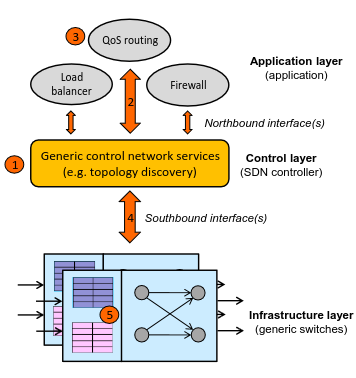
\includegraphics[width=0.5\textwidth]{pictures/4/SDN.png}
	\caption{Architettura SDN}
\end{figure}
\subsection{OpenFlow Switch}
Il termine switch viene usato in modo generico, in quanto non offrono solo funzionalità al livello 2.
In particolare analizziamo il paradigma di OpenFlow, che è uno dei primi e più diffusi standard per SDN.
\subsubsection{Control channel}
Gestisce la comunicazione con il controller, prende regole di flusso (o flow entries) specificate dal controller e le installa nelle flow tables.
In questa sezione ci riferiamo a flow come a un insieme di pacchetti che matchano lo stesso set di campi.
Inoltre, il control channel genera i messaggi da inviare al controller.
\begin{figure}[H]
\centering
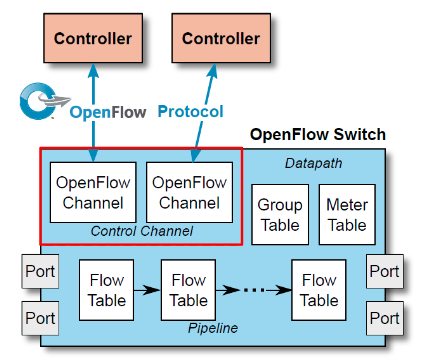
\includegraphics[width=0.5\textwidth]{pictures/4/OF_control_channel.png}
\end{figure}
\subsubsection{Tabelle}
Le tabelle di flusso vengono implementate come pipeline per migliorare le prestazioni, inoltre ci sono due tabelle speciali:
\begin{itemize}
	\item \textbf{Group table}: usata per implementare funzionalità avanzate come il multicast, il broadcast, il load balancing, ecc.
	Contiene gruppi di azioni che possono essere applicati a pacchetti che matchano con le flow entries.
	\item \textbf{Meter table}: acquisisce statistiche sui flussi di traffico e applica politiche di qualità del servizio (QoS) come il rate limiting.
\end{itemize}
\begin{figure}[H]
\centering
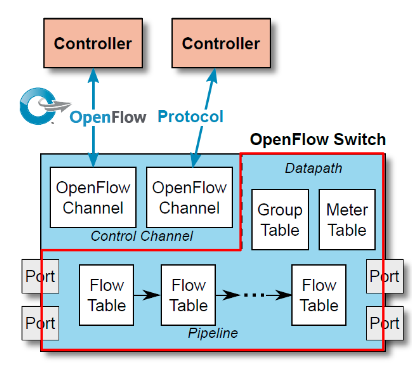
\includegraphics[width=0.5\textwidth]{pictures/4/OF_tables.png}
\end{figure}
\begin{figure}[H]
\centering
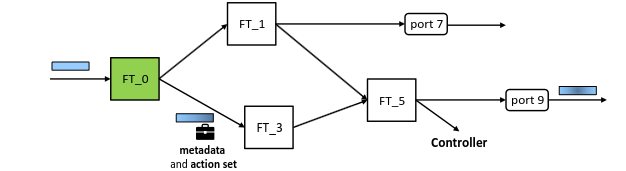
\includegraphics[width=\textwidth]{pictures/4/table_pipeline.png}
\caption{Esempio di pipeline di tabelle in un OpenFlow switch.}
\end{figure}
Nell'esempio della figura, solo FT\_0 è obbligatoria, le altre dipendono dalle funzionalità che si vogliono implementare.
Le entità che vengono allegate al pacchetto sono:
\begin{itemize}
	\item \textbf{Metadati}: informazioni rilevanti per il processing del pacchetto, non fanno parte dell'header del pacchetto ma vengono usati per prendere decisioni.
	\item \textbf{Action set}: lista di azioni che verranno effettuate più tardi nella pipeline eseguendo una determinata istruzione.  
\end{itemize}
Quindi per ricapitolare:
\begin{itemize}
	\item L'amministratore di rete scrive delle applicazioni che sfruttano le north bound interfaces per specificare il comportamento desiderato della rete (comandi ad alto livello).
	\item Il controller SDN traduce questi comandi in un insieme di regole.
	\item Le regole di flusso vengono installate nelle flow tables degli switch tramite le south bound interfaces.
\end{itemize}
\subsection{Tipi di configurazioni}
\begin{itemize}
	\item \textbf{Proattiva}: le tabelle di flusso sono sompletamente configurate da OpenFlow all'avvio dello switch. Tutte le entrate sono statiche e non sono modificabili a runtime.
	\item \textbf{Reattiva}: le tabelle di flusso sono configurate a runtime (sono vuote allo startup).
	Se un pacchetto arriva e non appartiene a nessun flusso, viene inoltrato al controller (packet-in message) che decide come gestirlo e installa una nuova regola di flusso.
\end{itemize}
Tipicamente gli switch lavorano in una modalità ibrida, con alcune regole di flusso preinstallate e altre che vengono installate a runtime.
Le regole preinstallate devono gestire buona parte del possibile traffico, in modo da minimizzare il numero di pacchetti che devono essere inoltrati al controller.
In generale, configurare le tabelle è un processo complesso, che richiede una buona conoscenza della rete e del traffico che la attraversa.
\subsection{SD-WAN}
È un approccio molto moderno (2014), che vuole ridurre i costi di una WAN usando principi SDN.
L'idea principale è quella di usare diverse connessioni a banda larga generiche con accesso a internet, in modo di garantire un certo livello di QoS.
\begin{figure}[H]
\centering
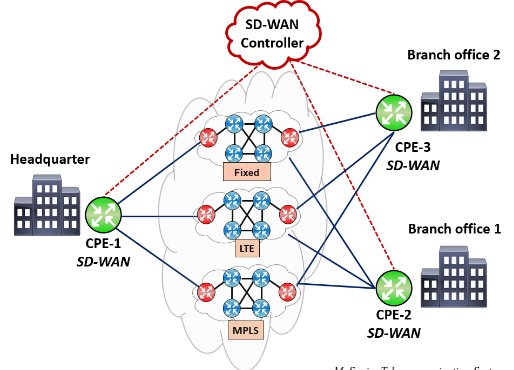
\includegraphics[width=0.5\textwidth]{pictures/4/SD-WAN.png}
\caption{Architettura SD-WAN.}
\end{figure}
I componenti principali di un'architettura SD-WAN sono:
\begin{itemize}
	\item \textbf{SD-WAN box}: presente in ogni sede (CPE, customer premises equipment).
	\item \textbf{SD-WAN controller}: gestisce i CPE e i flussi di traffico tra sedi.
\end{itemize}
Questa soluzione è molto più economica di MPLS e mantiene comunque buone prestazioni.
Può anche essere usata in modo ibrido, ad esempio per connettività intercontinentale.
\section{Data plane programming}
La rappresentazione logica della pipeline del piano dati non è flessibile, in quanto è necessario cambiare hardware per:
\begin{itemize}
	\item Un nuovo campo di matching deve essere supportato.
	\item Se un nuovo protocollo deve essere supportato.
\end{itemize} 
Con il \textbf{Data plane programming} abbiamo la possibilità di programmare la pipeline del piano dati dello switch.
In questo modo, possiamo programmare non solo il control plane, ma anche il data plane, ottenendo una flessibilità molto maggiore.
\subsection{PISA}
PISA (Protocol Independent Switch Architecture) e PSA (Programmable Switch Architecture) sono architetture di switch che supportano il data plane programming.
Gli header e i metadati possono essere usati per il matching, come in openflow, ma inoltre è possibile:
\begin{itemize}
	\item Personalizzare il parser di pacchetti.
	\item Definire flessibilmente la struttura delle tabelle.
	\item Modificare, rimuovere o aggiungere campi degli header.
	\item Eseguire azioni stateful.
\end{itemize}
\textbf{P4} è il linguaggio specifico standard de facto per il data plane programming.
\begin{figure}[H]
\centering
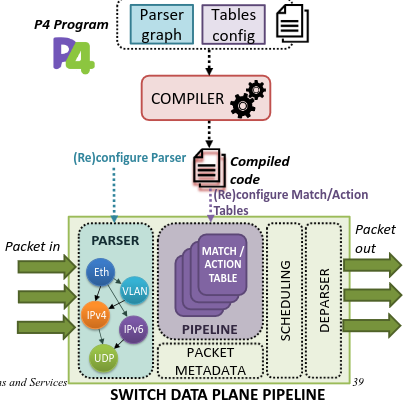
\includegraphics[width=0.5\textwidth]{pictures/4/P4.png}
\caption{Esempio di architettura con supporto al data plane programming.}
\end{figure}
\section{Network function virtualization}
Paradigma molto recente (2013), il NFV disaccoppia l'hardware dal software tramite implementazioni di funzioni di rete come software che gira su hardware generico.
In questo modo non è necessario avere hardware dedicato per ogni funzione di rete, ma è possibile eseguire più funzioni su un unico hardware condiviso.
Questo porta a costi minori, maggiore flessibilità e scalabilità.
Tuttavia, NFV è adatto per la virtualizzazione di funzionalità di piano di controllo, molto meno per funzionalità di piano dati.
Questo perché le funzionalità di piano dati richiedono prestazioni molto elevate, che non possono essere garantite da hardware generico.
In generale, le funzionalità del piano di controllo richiedono meno velocità (ma sono operazioni più complesse).
L'NFV è un primo passo verso la "cloudificazione" delle reti.